
\subsection{Software} \label{subsec:software}

In diesem Kapitel wird die Umsetzung der Software dokumentiert und wie die in den Grundlagen beschriebenen Themen eingebaut werden. Die Software ist nach dem MVC Framework (TODO:Verweis) aufgebaut. Das Klassendiagramm der Software befindet sich im Anhang (TODO: Verweis)
%TODO Verweis
\begin{figure}[H]
		\centering
		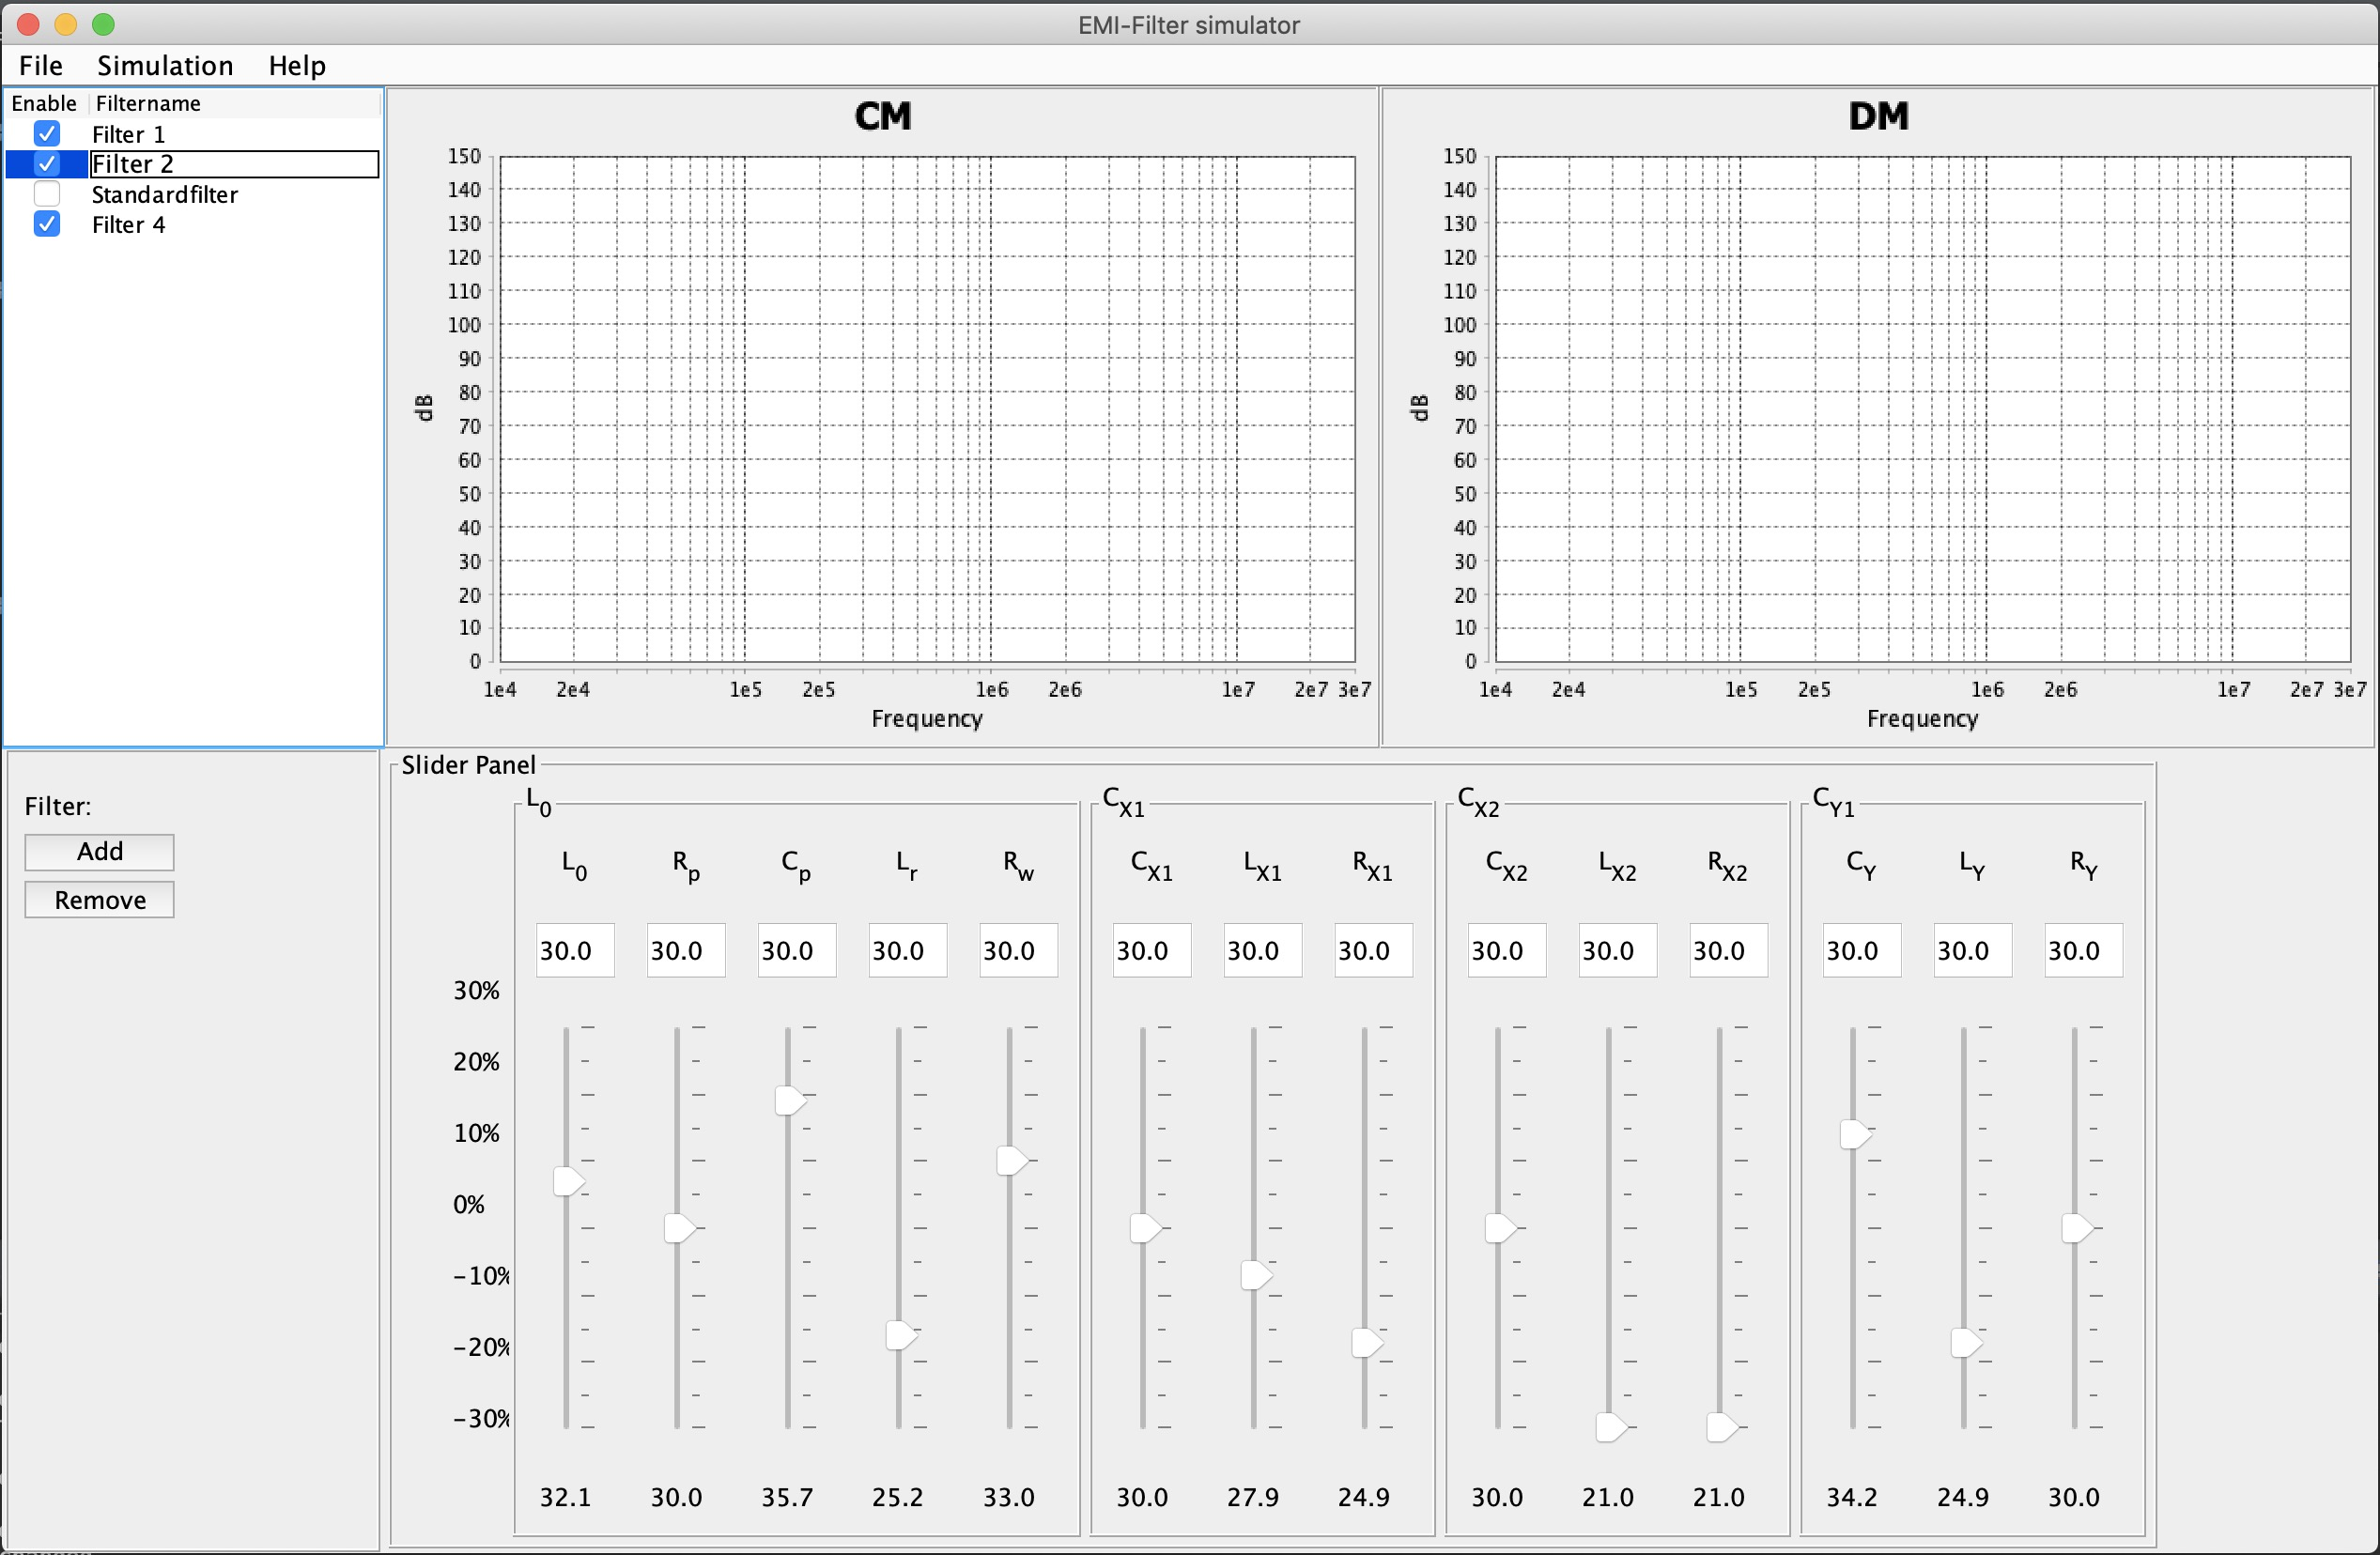
\includegraphics[width = 15cm]{GUI_unfertig.jpg}
		\label{fig:gui}
		\caption{Benutzeroberflächre unfertig}
\end{figure}

Die Oben abgebildete Benutzerfläche ist die Maske, welche sich beim aufstauten der Software auf dem Bildschirm präsentiert.
Wie die  meisten gängigen Applikationen verfügt die GUI eine am oberen Rand platzierten Menubar, um Dateien zu verwalten sowie Hilfestellung zu bieten.
Im Zentrum ist im oberen Bereich das Plotpanel platziert, welches die Simulation sowohl im Gleichtakt (CM), als auch im Gegentakt (DM) als grafische Kurve darstellt.
Gleich unterhalb befindet sich das Inputpanal, es ermöglicht mittels den Textfeldern eine  effiziente Eingabe der  Parameter. Mittels den Sleidern können die Parameter prozentual angepasst werden.
Die Filtertabelle links dient zur Verwaltung der Filterprofilen.


\subsubsection{View}\label{subsubsec:view}

Die View ist für die Darstellung der Daten und die Verarbeitung der Benutzereingaben zuständig. Zur View gehören die Panels: InputPanel (1), FiltertablePanel (2), ButtonPanel (3), Menubar (4) und PlotPanel (5). In diesem Abschnitt werden die Panels dokumentiert Diese bilden zusammen die Benutzeroberfläche, die in der Abbildung (TODO verweis) ersichtlich ist. Im Klassendiagramm (TODO Verweis Anhang) sind alle Klassen die zur View gehören, mit der Farbe (TODO: Farbe) markiert.

%TODO Bild
\paragraph{Menu} \label{par:menu}

Die Menübar verfügt über drei Menüs das File-,  Simulation- und ein Help-Menü.

Das File-Menü dient zur Datenverwaltung, es erlaubt Filterprofile mittels "Save" abzuspeichern und "Load" zu laden. 
Das Programm wandelt das Filterprofiel in ein Komma-getrenntes Textfile.

Mittels "Save" wird das angewählte Filterprofil abgelegt. Es öffnet sich ein Dialog-Fenster,ein File Chooser, dieser erlaubt es den gewünschten Speicherpfad auszuwählen und die Datei zu benennen. Die Eingabe wird mit "Save" bestätigt. Nun ladet das Programm den zugehörigen Array welcher das Filterprofil enthält, mithilfe des Printwriter in ein Textfile. Das Textfile wird nun unter dem gewünschten Pfad abgelegt. 

\paragraph{Inputpanel} \label{par:inputpanel}

\paragraph{Plotpanel} \label{par:plotpanel}

\paragraph{Filterpanel} \label{par:filterpanel}

\paragraph{Buttonpanel} \label{par:buttonpanel}


\subsubsection{Model}\label{subsubsec:model}

\subsubsection{Controller}\label{subsubsec:Controller}




